% Create subfigures in LaTeX
\documentclass{article}

\usepackage{subcaption}
\usepackage{graphicx}

\begin{document}

\begin{figure}

\centering
\begin{subfigure}{0.48\textwidth}
    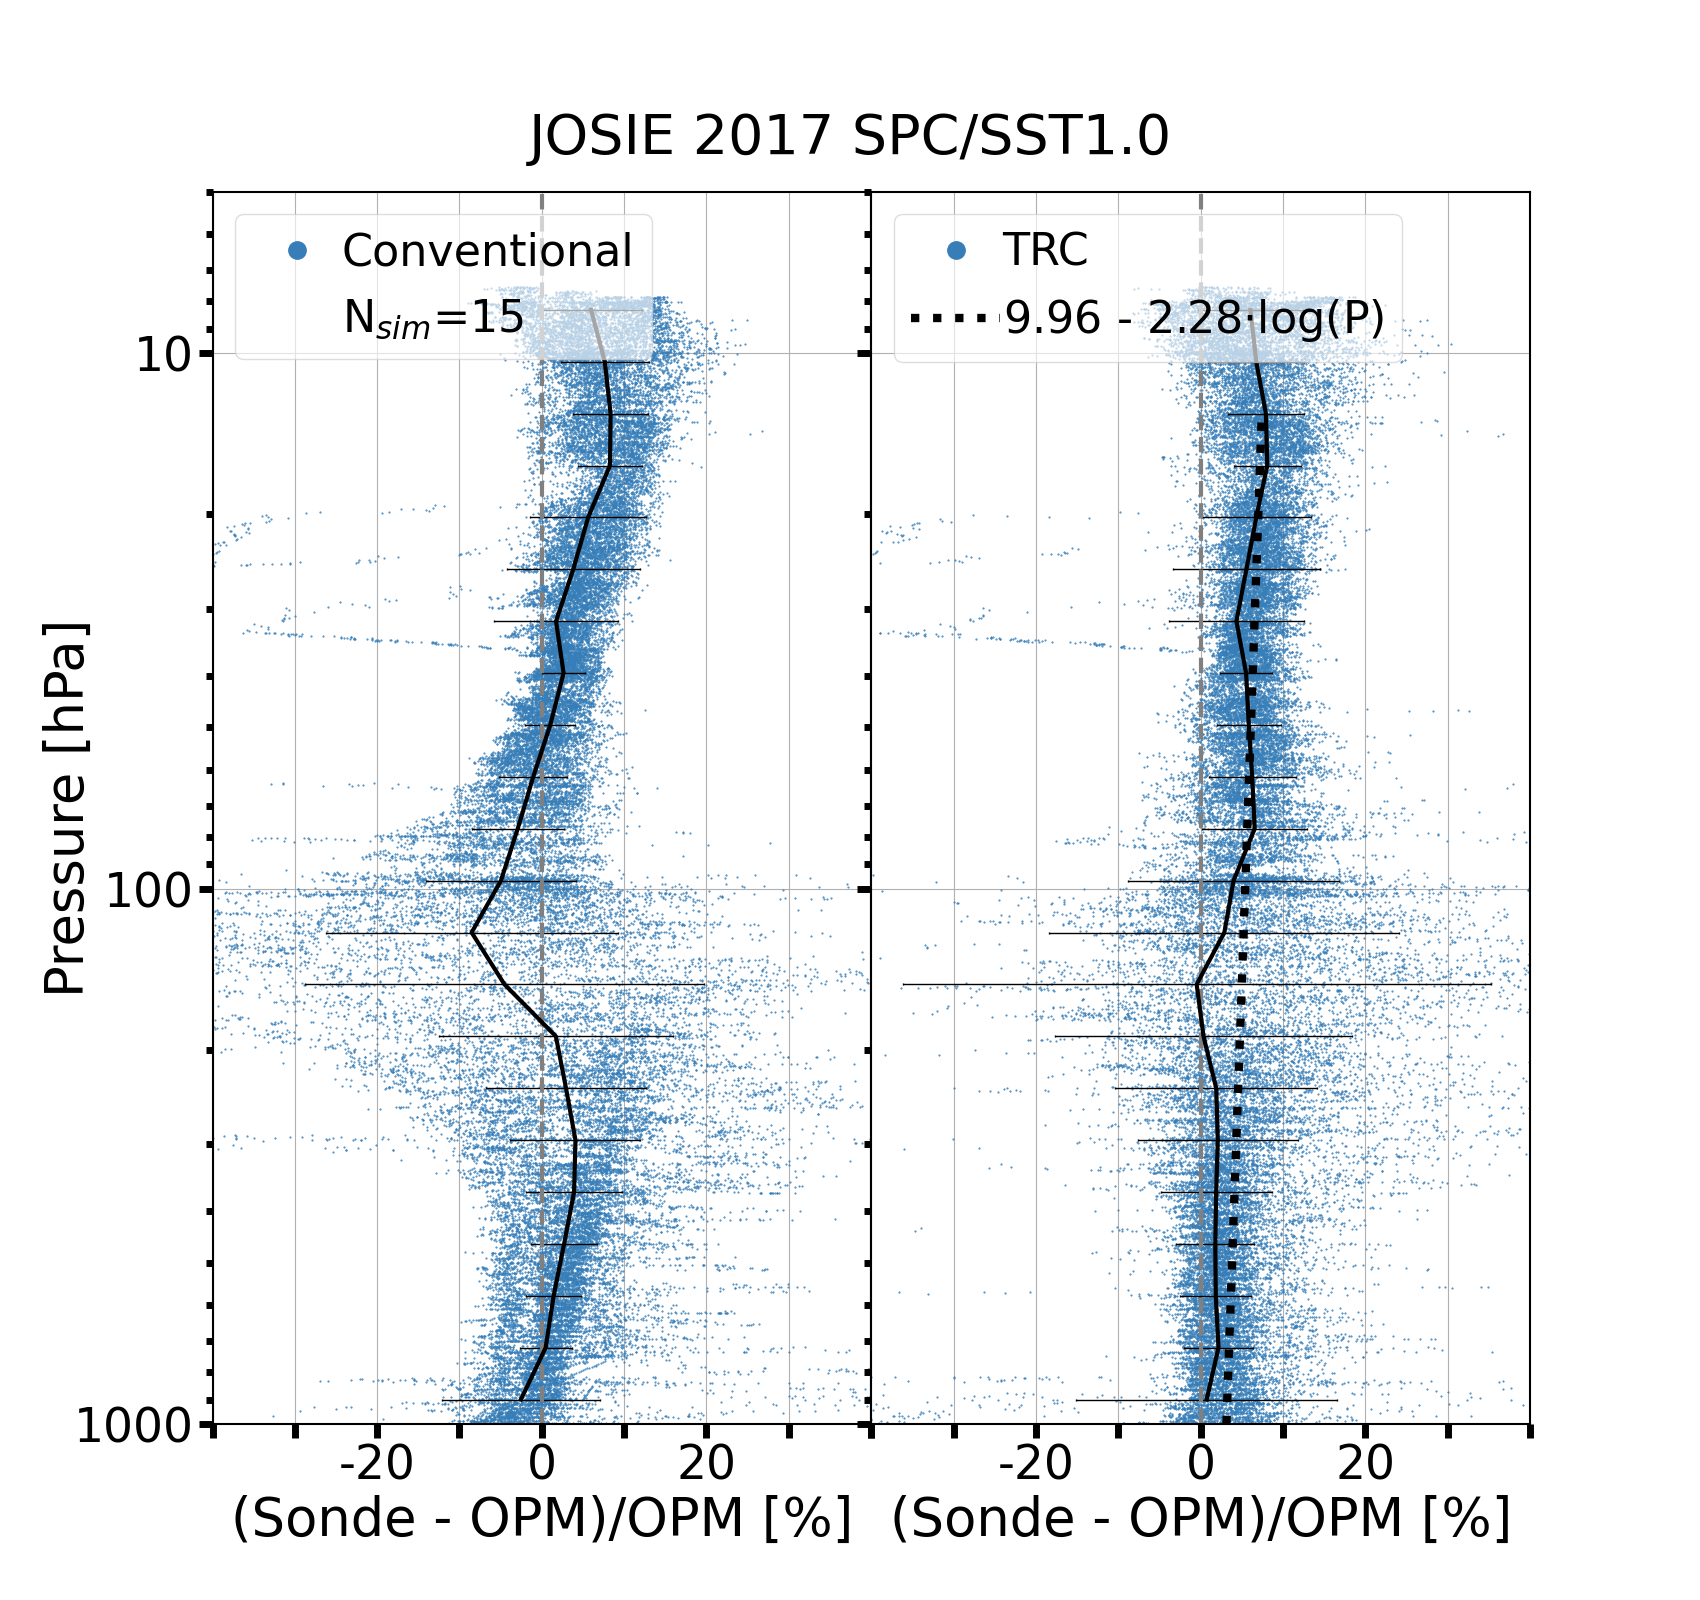
\includegraphics[height = 0.45\textheight,width=\textwidth ]{png/scatter_2017_SPC1010_pressure}
%    \caption{Firts subfigure.}
%    \label{fig:first}
\end{subfigure}
\hspace{0.01mm}
\begin{subfigure}{0.48\textwidth}
    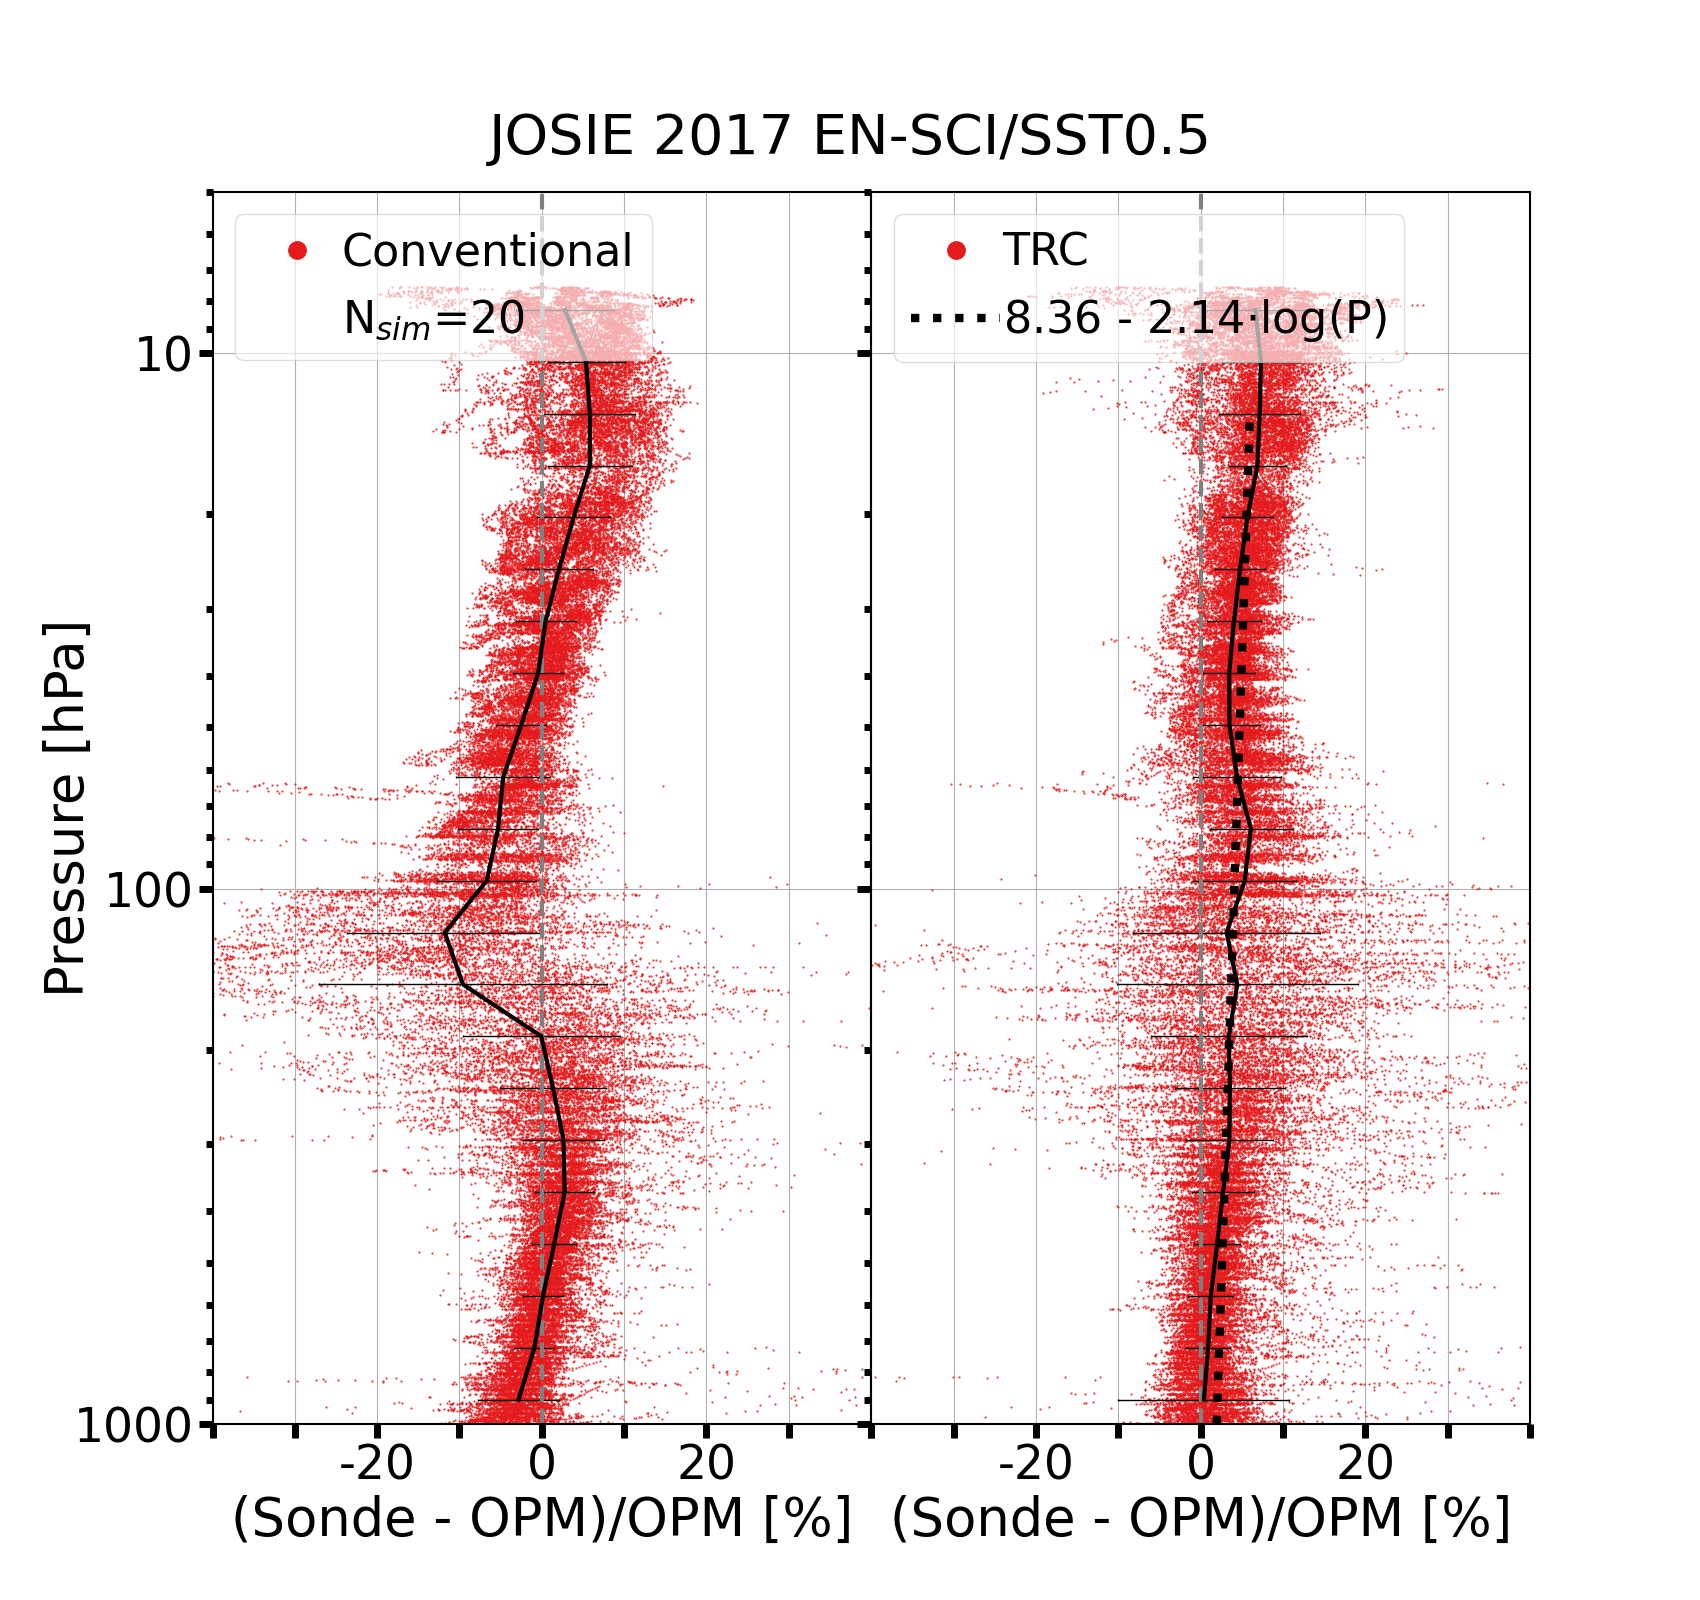
\includegraphics[width=\textwidth]{png/scatter_2017_EN0505_pressure}
%    \caption{Second subfigure.}
%    \label{fig:second}
\end{subfigure}
\hspace{5mm}

%\begin{subfigure}{0.4\textwidth}
%    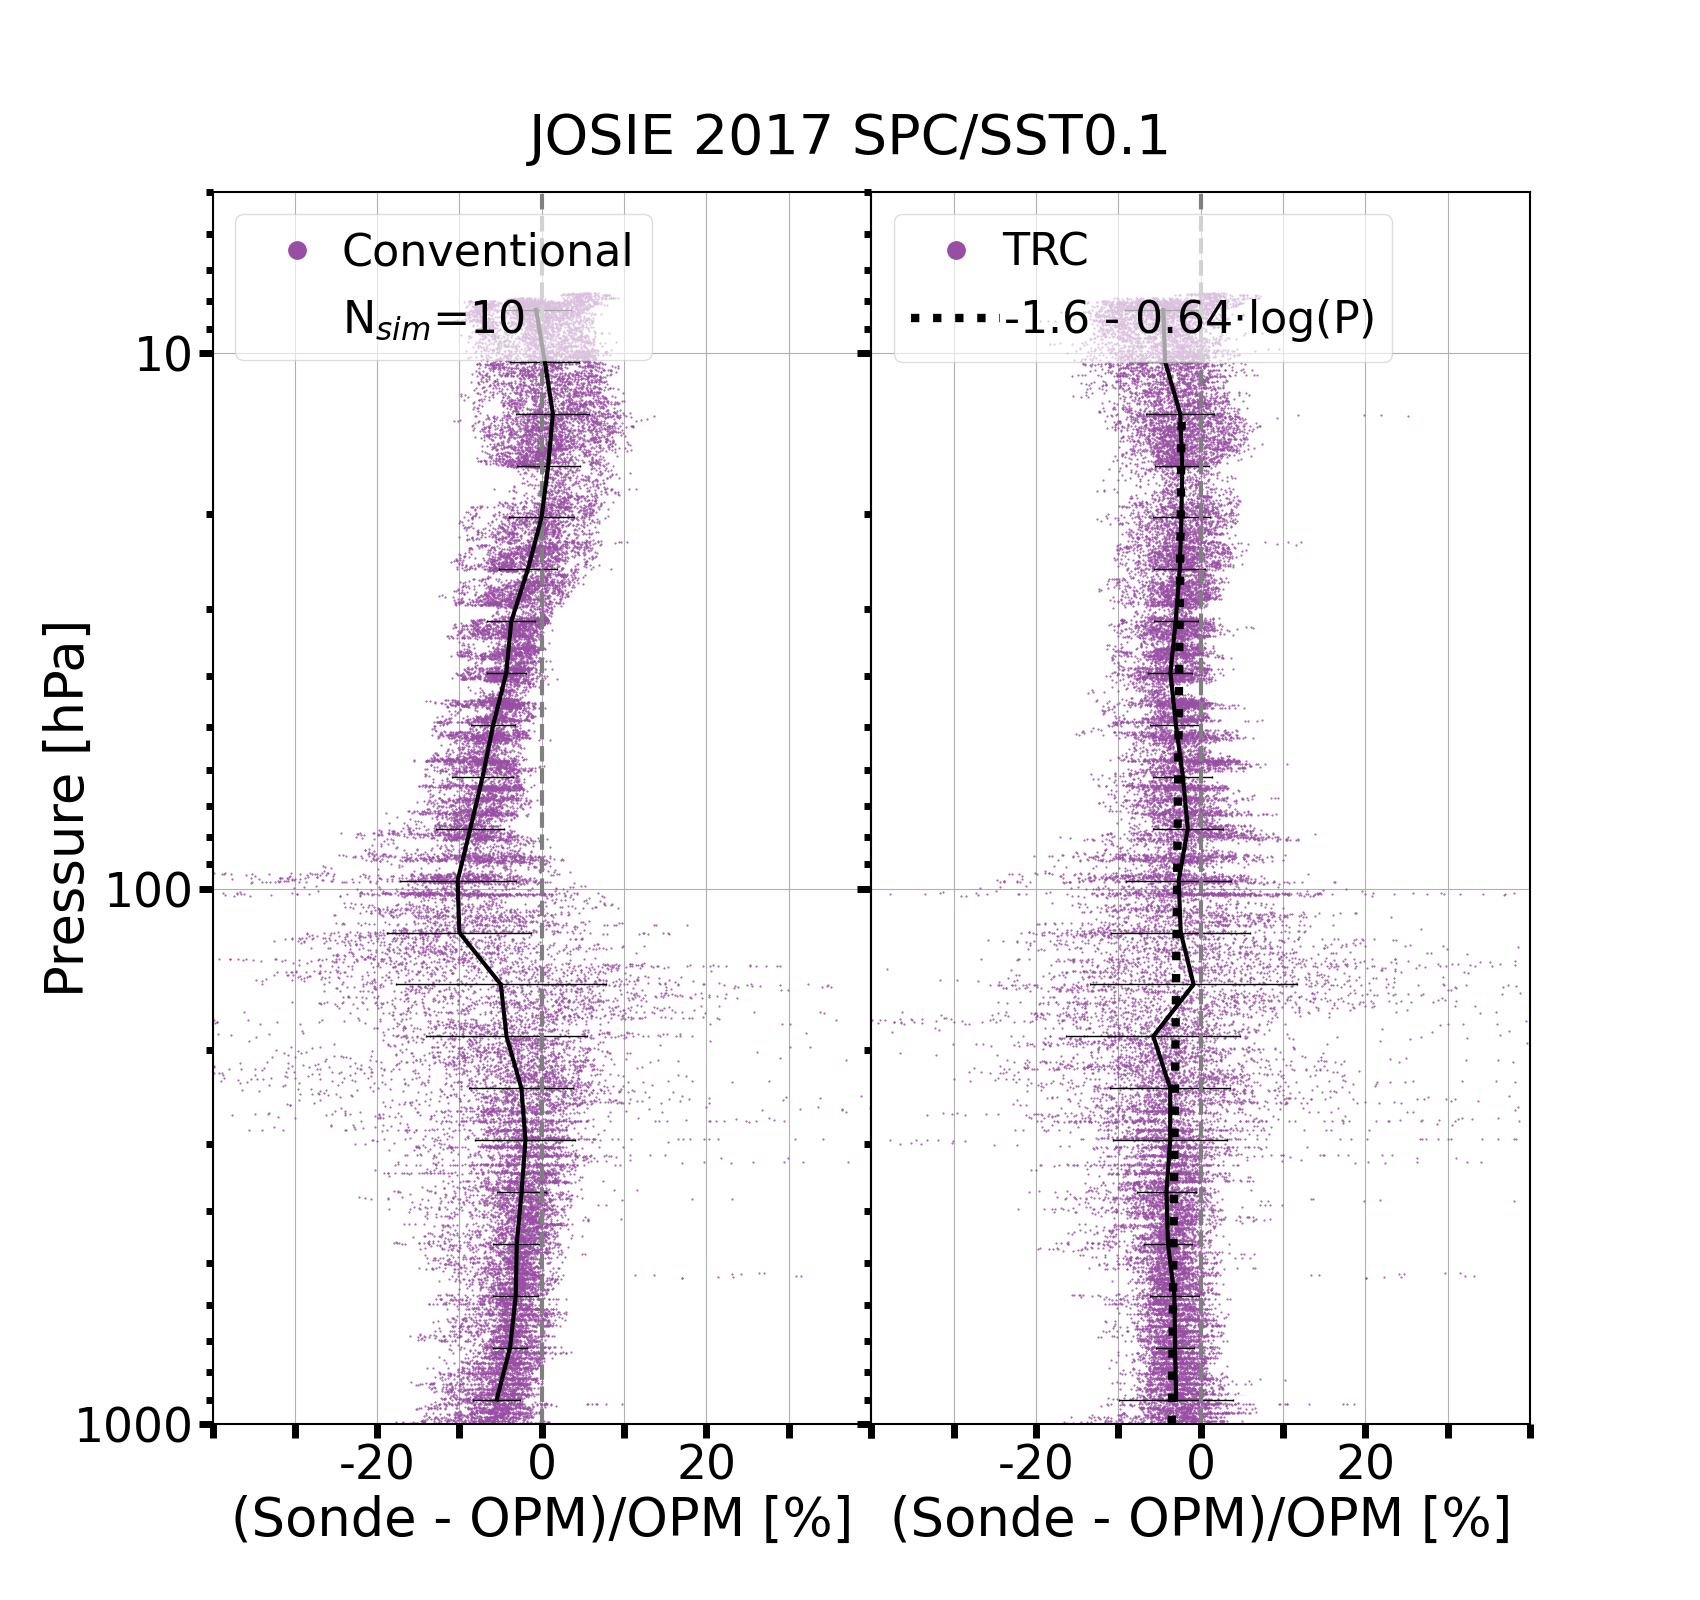
\includegraphics[width=\textwidth]{png/scatter_2017_SPC1001_pressure}
%%    \caption{Firts subfigure.}
%%    \label{fig:first}
%\end{subfigure}
%\hfill
%\begin{subfigure}{0.4\textwidth}
%    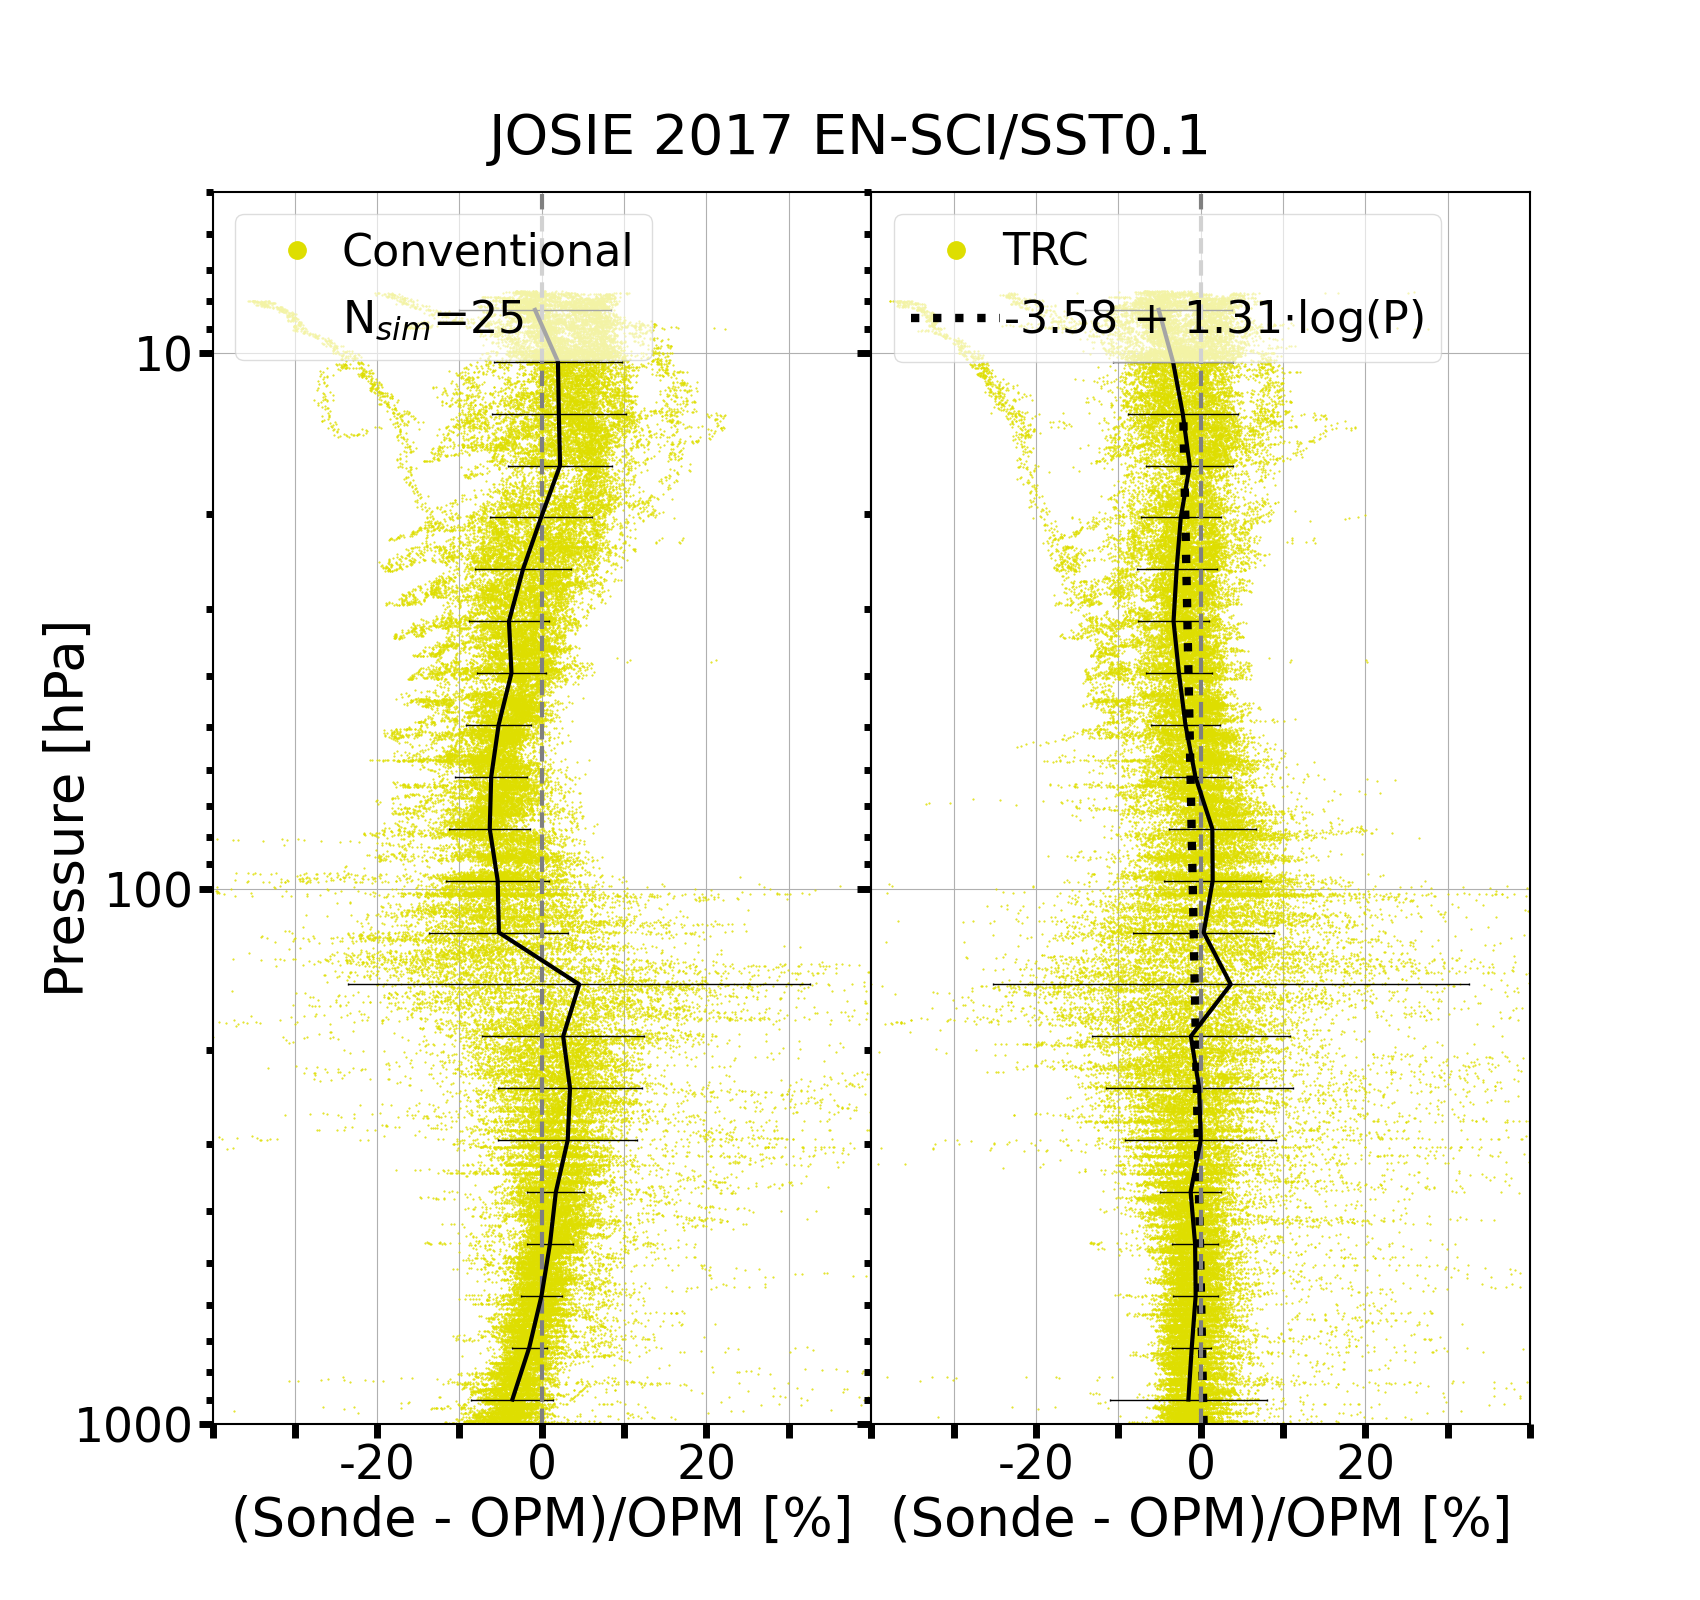
\includegraphics[width=\textwidth]{png/scatter_2017_EN1001_pressure}
%%    \caption{Second subfigure.}
%%    \label{fig:second}
%\end{subfigure}

%\caption{Creating subfigures in \LaTeX.}
\label{fig:figures}

\end{figure}

\end{document}